% This is LLNCS.DEM the demonstration file of
% the LaTeX macro package from Springer-Verlag
% for Lecture Notes in Computer Science,
% version 2.4 for LaTeX2e as of 16. April 2010
%
\documentclass{article}
%
\usepackage{makeidx}  % allows for indexgeneration
\usepackage{color} %vrivas, 15-Jan-2016
\usepackage{hyperref} %vrivas, 21-Jan-2016, for \url
\usepackage{graphicx} %vrivas, 27-Jan-2016, for images
\usepackage{listings}%vrivas, 27-Jan-2016, for code
\usepackage{algorithm} %jj, dec-8-2016, for code
\usepackage{algorithmic} %jj, dec-8-2016, for code
\usepackage{authblk} %jj, dec-20-2016, for authors

\begin{document}
%

\title{Time series forecasting using evolutionary neural nets implemented in a
  volunteer computing system}
%Nuevo t�tulo propuesto. 
%

% Author according to authblk
\author[1,3]{V.M. Rivas}
\author[1]{E. Parras-Guti\'{e}rrez}
\author[2,3]{JJ Merelo}
\author[2,3]{M.G. Arenas}
\author[4]{P. Garc\'{\i}a-Fern\'{a}ndez}

% Affiliations according to authblk
\affil[1]{Univ. of Jaen, Dept of Computer Sciences,\\
Campus Las Lagunillas s/n, 23071, Ja\'{e}n, SPAIN\\
\texttt{vrivas@ujaen.es}, 
\texttt{http://vrivas.es}}

\affil[2]{Depto. de Arquitectura y Tecnolog\'{\i}as de las Computadoras\\
Univ. de Granada, SPAIN
Univ. of Granada, Dept. of Computers, Architecture and Technology,\\
C/ Periodista Daniel Saucedo s/n, 18071, Granada, SPAIN}

\affil[3]{GeNeura Team \\
  \url{http://geneura.wordpress.com}
}

\affil[4]{Depto. de Electr\'{o}nica y Tecnolog\'{\i}as de las
  Computadoras\\
 Univ. de Granada, SPAIN
 Univ. of Granada, Dept. of Electronics and Computer Technology}

\maketitle              % typeset the title of the contribution
\begin{abstract}
%##### NUEVA PROPUESTA DE ABSTRACT--- Maribel
{\em JsEvRBF} is a forecasting method that uses a genetic algorithm
for evolving radial basis function neural nets. The implementation
presented in this paper is able to run in most modern web browsers,
consequently everybody is allowed to contribute the algorithm
results participating in the experiments using their own browsers. The
use of browsers for experimentation is an interesting idea because the
scientists could use the huge number of inactive web browsers included
in each device as computation power, but it is a great challenge
too because the language support and performance varies as the
JavaScript Virtual Machine implementation changes hampering the same
algorithm is run in the same version or each browser.
The presented
results include a description of the experimentation process using
volunteers, which is one of the goals of this paper, and the
forecasting results using a currencies exchange dataset which are
comparable with previous results without the volunteer
participation. These results guarantee the viability of the proposal. 

%#### cuando tengamos nuevos resultados puedo concretar un poco m �s la �ltima frase, que la he dejado un poco ambig�a
% You can't say "the presented results do this". Say what you intented
% to prove and to what extent it has been proved.
% And please check below for the classical structure of an abstract:
% motivation, objective, methods, advance on results - JJ

%This paper presents the implementation of a time series
%forecasting algorithm, {\em jsEvRBF}, that uses genetic algorithm and neural nets
%in a way that can be run in must modern web browsers. Using browsers to run forecasting algorithms is a challenge,
%since language support and performance varies across implementations
%of the JavaScript virtual machine and vendor. However, their use will
%provide a boost in the number of platforms available for
%scientists. % A bit of motivation for the paper
%% Papers need to have: motivation, objective. And the first sentences
%% in the paragraph will have to go in that direction.
%{\em jsEvRBF} is
%written in JavaScript, so that it can
%be easily delivered to and executed by any device containing a
%web-browser just accessing an URL. The experiments show the results
%yielded by the algorithm over a  data set related to currencies
%exchange. % the results are what? Good? Better? Worse?
%Best results achieved  can be effectively compared against
%previous results in literature, though robustness of the new algorithm
%has to be improved. % What was your objective? Just running it?
%                    % Running it with a decent performance? - JJ

\end{abstract}
%
\textit{Keywords}: Time-series forecasting, evolutionary computation, radial basis function neural networks, Web-based programming, volunteer computation

\section{Introduction}
% Web-based computing
Web browsers stopped to be just simple HTML renderers at the moment
they allowed the executions of third-part programs included in the
pages they downloaded. This way, browsers turned into wider
frameworks in which multi-platform applications could be executed.  
Flash??? reference??? and Java applets the??? are probably the best
known techniques to do this, even for non-experts users. But, in
%fact,  
Nowadays, most programs executed by browsers are written in a language
called JavaScript, which was initially introduced to make interaction
with web pages more similar to what was available in desktop
applications \cite{Rauschmayer04}. % Don't know about this
                                % reference. Isn't it too recent? - JJ
                                
                                
% CITA En la que dice que Flash se dej� de usar en favor de HTML por el mismo Adobe                                Winokur, D. (2011). Flash to focus on PC browsing and mobile apps; Adobe to more aggressively contribute to HTML5. Retrieved, September 26, 2013 from http://blogs.adobe.com/conversations/2011/11/flash-focus.html
% Add to bibliography if needed - JJ

Current everyday massively-used web pages and web applications (including those related to social networks) exist thanks to this language.
Its use has turned browsers into wider frameworks in which multi-platform applications can be run.
%The web, as we currently use it, would not be the same without the
%capability that JavaScript gives to the browser to make calculus,
%interact with the user, or dynamically retrieve data from servers
%without reloading the whole page, as it's done with AJAX
%Reference???.  
%Throughout the 1990s, the proprietary web browser Netscape Navigator had been created and was dominant, and in 1995, Brendan Eich was hired by Netscape company to design and implement a new language. At the same time, Netscape collaborated with Sun company to include in Navigator Java, its more static programming language, so it was questioned the needed of two programming languages: Java and a scripting language. Finally, they decided that the new scripting language had to make more accessible to non-Java programmers and web designers the support for Java applets \cite{Champeon08}. In May 1995, Eich designed a prototype in 10 days and was named first \emph{Mocha}, coined by the founder of Netscape Marc Andreessen, then \emph{LiveScript} and finally, in December 1995, \emph{JavaScript} \cite{Eich2010}, not because of the Java programming language, but to support Sun Microsystems.
JavaScript was standardized in 1997 by the European Computer Manufacturer's Association, or ECMA. According to the ECMA-262 standard, its real name is \emph{ECMAScript}, but everyone calls the language \emph{JavaScript} \cite{Flanagan06}.

% Restricciones de JavaScript
JavaScript can be described as a general-purpose, object-based, event-driven language.
% that can be used to write programs for both the client and the
% server REFERENCE-NODE???. T�
% Why comment??- JJ
Adding JavaScript programs to web pages is simple: the code is inserted in the HTML code in plain text; then, it is downloaded by the browser that, finally,  interprets and executes it.
%Thus, although web browsers allow the users to change the preferences
%in order to disable the execution of any JavaScript code, this is
%rarely done in these days. Even more, most standard web users are not
%aware of the existence of this language, not realizing their browsers
%are working as programming environments in which code is analyzed,
%translated into a low-level language and executed. Consequently, and  
%For safety reasons, programs written in JavaScript are executed by
%browsers using a sandbox model. This model imposes a series of
%restriction that could be summarized as: the JavaScript program
%inserted in a given web page cannot access any other resources than
%the ones contained in that web page. JavaScript programs are allowed
%to the client's file system to store little pieces of text (called
%cookies), and also when the user has to select a file to be sent
%across the net. 
Due to the capabilities of JavaScript, in this work we propose the use
of web browsers as agents able to download a web page containing a set
of data, execute an evolutionary algorithm that evolves neural nets,
and apply this neural nets to forecast an economic time-series. Using
this approach, any device  able to execute a web browser (from
computers to smart TVs) can be potentially used to run our algorithm. 

% Genetic Algorithms and RBFNN
Both the problem being considered in this paper and the algorithm used
to solve it were introduced in \cite{rivas03:EvRBF}. On the one hand,
the problem consists on forecasting the values of the exchange rates
between two currencies for a four years period; data is averaged
weekly. %This needs a citation. Where did you obtain data?
% Besides, could you use our own traffic data? - JJ
On the other hand, the algorithm (described in
section \ref{sec:algorithm}) is a reduced version of {\em EvRBF}
\cite{rivas03:EvRBF}, an evolutionary algorithm that makes Radial Basis
Function Neural Networks (RBFNN) to evolve.
% Now you're talking. You should say exactly what you have reduced,
% and make a more extensive description of EvRBF - JJ

RBFNN are well-known feed-forward neural nets with just one hidden and
one output layers. %\cite{Broomhead88}.  
They have been successfully used to solve classification, function
approximation, and, as in this work, time-series forecasting problems
\cite{Broomhead88,Keogh03,Whitehead}. 
%The neurons in the output layer (only one neuron in this work) compute a weighted sum using outputs provided by hidden neurons, multiplied by some weights previously established, and adding a bias. The neurons in the hidden layer receive the input samples concerning the problem being resolved, and apply an activation function that  is a Radial Basis Function, i.e., a function returning a value that depends on the distance from the input values to a pre-established center of the function. The shape of this function is modified by means of a radius or width: the narrower this width, the higher the number of inputs that will not activate the neuron. Usually, Gaussian function is selected as the activation function, but many others can also be used.
Configuring an RBFNN in order to solve a task consists on: a) choosing the activation function for hidden neurons, b) choosing the number of hidden neurons, c) setting the parameters required by the activation functions (i.e., center and radius of the RBF), and d) setting the values for weights and bias. This last step can be easily computed once the rest of components have been established using the Least Mean Square method. {\em EvRBF} algorithm was designed to automatically search for the best configuration of an RBFNN that solves the problem being tackled, except for the activation function to be used that is always a Gaussian function.

% Time-series prediction

%Time-series can be considered as a special kind of function approximation where future values of the series are expressed as a function of past ones.
%There exist many methods in literature developed to forecast time-series references, being ARIMA \cite{BoxJenk} probably the most widely used.

In the herein, the implementation of {\em EvRBF} for web browsers
(called {\em jsEvRBF}) has been compared to its original
implementation as well as to the methods used by Sheta in
\cite{Sheta2001}, the work in which the data set used in this paper
was introduced.

The rest of the paper is organized as follows: the state of the art in
distributed computing for financial prediction is presented in the
next section; our approach to this problem follows in Section
\ref{sec:algorithm}; the experimental setup to test our method and its
results are presented in Section \ref{sec:experiments}, and finally
and conclusions are drawn and future
lines of work presented in Section \ref{sec:conclusions}.

\section{State of the art}

Prediction of time series, specially financial ones, is considered a
hard problem requiring a great amount of computational resources,
since the model space that is explored is generally huge, so parallel
computing has been used at the same time than Genetic Programming,
\cite{santini2001genetic}, a technique that evolves rules and
expressions or neural networks \cite{niska2004evolving}, in which case
the parallel implementation is used to explore more efficiently the
space of different parallel architectures.

This is probably the reason why it has not been approached using
volunteer computing, which eschews fixed computing infraestructures,
relying on the computing resources lent by strangers
\cite{daniel:euromicro09,gecco07:workshop:dcor,DBLP:journals/corr/abs-0801-1210,DBLP:conf/gecco/MereloCGCRV16,baratloo1996charlotte,hwang2009determinants,web:BOINC}. Although
in these kind of networks a high sustained performance is difficult to
achieve \cite{DBLP:conf/lion/LaredoGFMACG11}, in the short term a
  good performance is achievable, with the only cost of setting up the
  experiment. That is why it has been applied successfully to protein
  structure prediction \cite{taufer2006predictor} and other
  experiments launched from the BOINC platform \cite{boinc_grid04}. In
  general, success has been met with the constraints of the difficulty
  in predicting the true performance of the meta-computer created by
  the experiment and its volunteers \cite{Merelo2016}. In fact, one of
  the major applications of non-volunteer computing in financial
  technology seems to be {\em illegal} bitcoin mining using the
  resources of infected computers \cite{plohmann2012case}. 

We have already published the proof of concept and preliminary results
for this method in \cite{DBLP:conf/dcai/RivasPMAG16}. In this paper we
correct errors found and describe further experiments that measure the
performance obtained with different browsers and in different
conditions. 


\section{The {\em jsEvRBF} algorithm} %Is it an algorithm or an
                                %implementation? - JJ
\label{sec:algorithm}
% The {\em EvRBF} general skeleton
{\em jsEvRBF} is an evolutionary algorithm written in JavaScript, so
that it can be executed in web browsers.
%Once again, you are mixing implementation and algorithm. Is it an
%algorithm or an implementation? ~ JJ
As in {\em EvRBF}
\cite{rivas03:EvRBF}, its predecessor, individuals are complete RBFNN, and
special operators have been created to cross and mutate them. %The
                                %same special algorithms or others? - JJ
{\em
  jsEvRBF} is a generational algorithm, with a fixed number of
individuals, that uses tournament selection and elitist
replacement\footnote{The code can be downloaded or forked from
  \url{http://bit.ly/jsEvRBF}; its use is restricted under the terms
  of the Apache 2.0 license.}. 

In order to implement both the RBFNN and the evolutionary algorithm,
two JavaScript libraries: {\em
  jsRBFNN}\footnote{\url{http://bit.ly/jsRBFNN}} and {\em
  jsEO}\footnote{\url{http://bit.ly/js-EO}}, have been developed by
our research group. {\em jsRBFNN} implements the neural nets and also the LMS
training algorithm. %This should be explained somewhere. This is a
                    %financial journal - JJ
{\em jsEO} \cite{EvoStar2014:jsEO} is a more
complex framework that allows the generation of many kinds of
evolutionary algorithms, making easier the task of creating new types
of individuals and/or operators. Figure \ref{fig:class_diagram}
graphically shows the dependencies between {\em jsEvRBF} and these
libraries.  


As a standard evolutionary algorithm, the skeleton of {\em jsEvRBF} is the following:

\begin{algorithm}
\caption{jsRBF program}
\begin{algorithmic}
\STATE Create, train and evaluate an initial population of $p$ individuals.
\FOR{generation = 1 \TO n}

   \STATE{Select a subpopulation of $q$ individuals}
   \STATE{Create $q$ new individuals applying an operator to each one in subpopulation}
   \STATE{Train and evaluate the $q$ new individuals}
   \STATE{Join and sort both old and new populations}
   \STATE{Remove the $q$ worst individuals}
\ENDFOR
\STATE Send the forecasting done by the best individual in last generation to the server
\end{algorithmic}
\end{algorithm}

\begin{figure}[!ht]
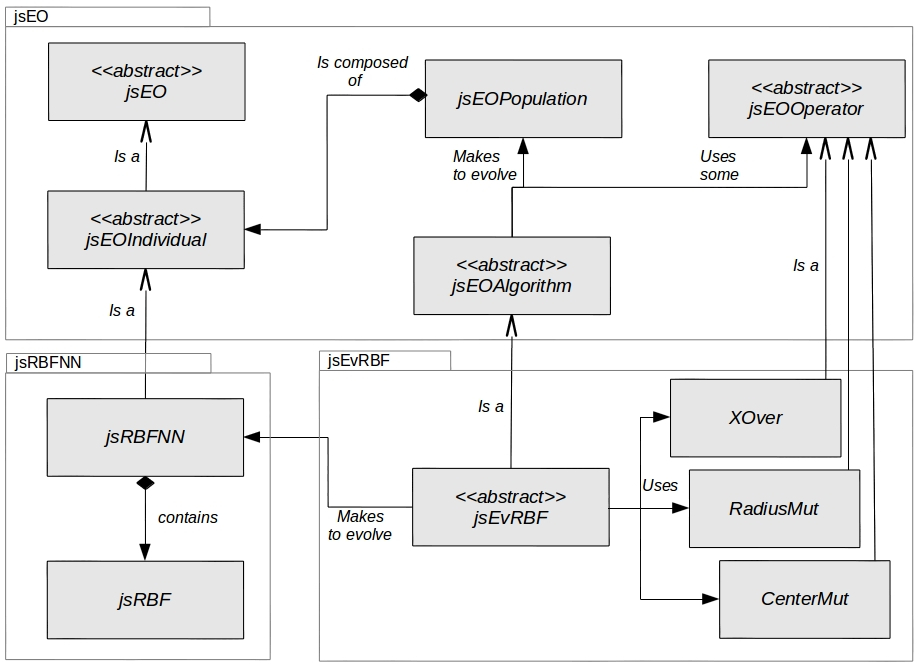
\includegraphics[width=120mm]{class-diagram.jpg}
\caption{Class diagram of the jsEvRBF algorithm, showing the way it depends on the jsEO general framework and the jsRBFNN library.}
\label{fig:class_diagram}
\end{figure}


%The individuals are RBFNN, any of them composed of a set of hidden neurons implemented as a vector of objects. Every hidden neuron stores its center and radius, and the global RBFNN stores the weights and bias. 
The fitness is computed using the inverse of the RMSE, so the greater the fitness, the better the individual. 

With respect to the operators used in this algorithm:

\begin{itemize}
\item {\em XOver.} Takes two individuals as inputs and operates by randomly selecting a set of neurons from first individual and another set (probably of a different size) from the second one. After this, those sets are interchanged.
\item {\em CenterMut.} Modifies a percentage of the centers of one individual setting them to random values in the range defined by the input dimension.
\item {\em RadiusMut.} Quite similar to the precendent, this operator modifies a percentage of the radius of the neurons of one individual, choosing a new value in the same way the {\em CenterMut} operators does.
\end{itemize}


Finally, the following set of parameters has to be established in order to run the {\em jsEvRBF} algorithm:
\begin{itemize}
\item{\em trnSamples}: Set of samples to train the nets; it will be also used to select the centers of the RBF of the individuals composing the initial population.
\item{\em valSamples}: Set of samples to compute fitness.
\item{\em inputDimension}: Dimension of inputs.
\item{\em numNeurons}: Number of neurons for individuals of the first population.
\item{\em popSize}: Number of individuals per population.
\item{\em numGenerations}: Number of generations for the evolutionary algorithm.
\item{\em tournamentSize}: Number of individuals to consider when selecting one of them to reproduce.
\item{\em replaceRate}: Rate of individuals to be replaced in every new generation.
\item{\em xOverRate}: Determines the number of individuals to which xOver operators will be applied.
\item{\em mutRate}: Determines the number of individuals to which mutator operators will be applied.
\item{\em mutPower}: Determines the number of neurons that will be changed by mutator operators, when applied to an individual.
\end{itemize}

Next section shows the values used for these parameters along the execution of the experiments.
% Specific characteristics of this implementation
% Operators
\section{Experiments and results}
\label{sec:experiments}
% The data-set
The {\em jsEvRBF} algorithm has been evaluated with the time-series
used by Sheta and de Jong \cite{Sheta2001}. %These kind of claims
                                %should go to the state of the art - JJ
It is composed of 208
weekly averaged observations representing the exchange rates between
Bristish pound and US dollar from 31 December 1979 to 26 December
1983\footnote{The source of the information, thanks to the work done
  by Prof. Werner Antweiler from the University of British Columbia,
  Vancouver, Canada, is available from
  \url{http://pacific.commerce.ubc.ca/xr/data.html}.}. This data set
has been used in a similar way than Sheta and de Jong: only half the
data (randomly chosen) has been used to train and validate the nets,
but the generalization error has been computed over the whole data
set. 

Two experiments have been carried out using {\em jsEvRBF}. One of them
has been open to a wide community of users, so that many different
devices, operating systems and web browsers have been used.  We have
also tested the algorithm in a single computer, using a single web
browser, so that we can focus in the forecasting process itself and
also assess the differences among different browser. 
In any case, participating in the experiment only required to connect
to an URL; no special technical knowledge was necessary to run the
algorithm since it was automatically executed once the web page was
loaded. Figure \ref{fig:example-of-execution} shows the page users
could read when accessing the specified URL.  As can be seen, it
emulated the look of a paper and needs no action to be performed by
the user.

Information about clients and the results they yielded were received
by a server programed also in JavaScript (using {\em node.js}) and
stored in a No-SQL database managed by {\em Mongo}; the language to
query the database was JavaScript too. The proof of concept results
have been published in \cite{DBLP:conf/dcai/2016de}; they showed some
promise of the method, as well as significant differences among
browsers. In this paper we report a new set of experiments and update
single-browser performance with updated browser versions. 


\begin{figure}[!ht]
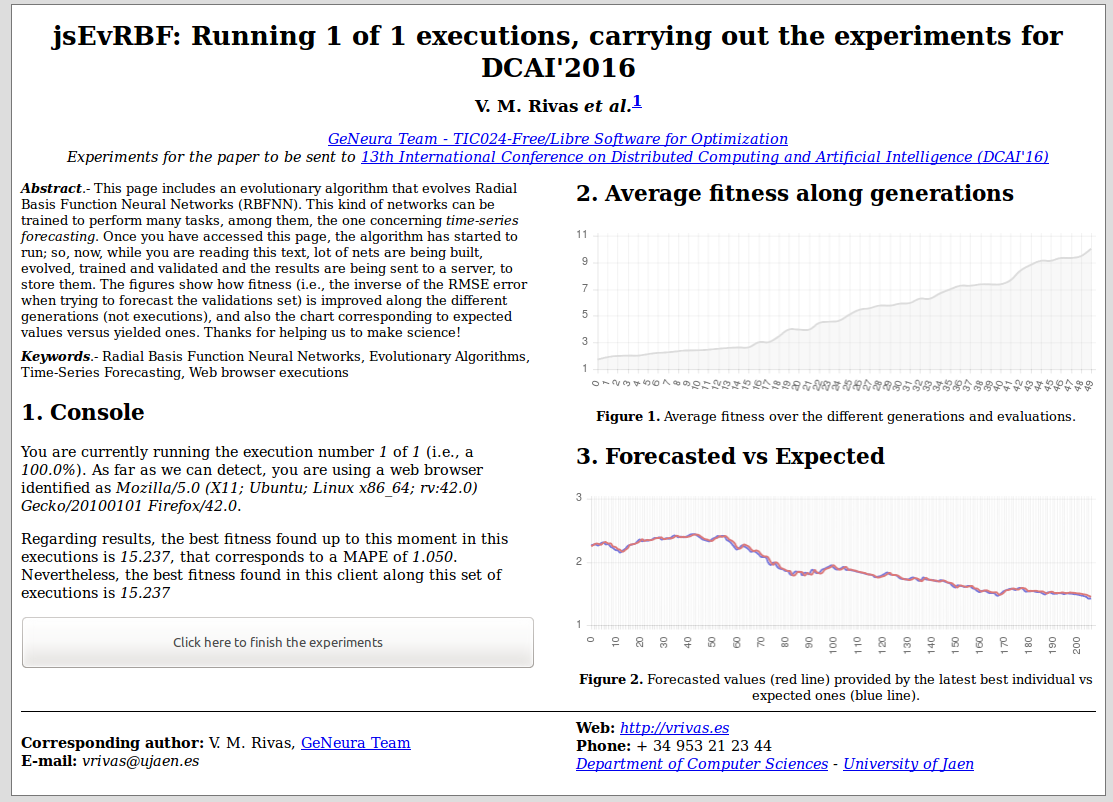
\includegraphics[width=120mm]{example-of-execution.png}
\caption{The look of the web page in which the {\em jsEvRBF} algorithm was loaded and executed.}
\label{fig:example-of-execution}
\end{figure}
% Maybe add new version of this screen - JJ

% Second one: only one browser, complete executions
\subsection{Testing single-browser performance}
\label{sec:second-experiment}

Once detected the error introduced by AppleWebKit-based browsers, a second experiment was carried out in a more controlled environment, and with a configuration similar to the original experiments in \cite{rivas03:EvRBF}. These new executions were run using a Firefox 44 browser, and configured as showed in table \ref{tab:parameters-second-experiment}.

\setlength{\tabcolsep}{10pt}
\begin{table}
\caption{Configuration of parameters for the second experiment. As in the first one, the number of samples ({\em trnSamples} and {\em valSamples}) is still approximated since they were randomly chosen in every execution. Values that differ from experiment 1 have been highlighted in {\bf bold}}
\label{tab:parameters-second-experiment}
\begin{center}
\begin{tabular}{rr|rr}
{\bf Parameter} & {\bf Value} & 
{\bf Parameter} & {\bf Value}\\
\hline
{\em trnSamples} & $\approx 90$ &
{\em valSamples} & $\approx 15$  \\
{\em inputDimension} &   1 &
{\em numNeurons} &  {\bf 10} \\
{\em popSize} &  {\bf 15} &
{\em numGenerations} & 10  \\
{\em tournamentSize} &  {\bf 3} &
{\em replaceRate} &   {\bf 0.2} \\
{\em xOverRate} &  {\bf 0.2}&
{\em mutRate} &   {\bf 0.8}  \\
{\em mutPower} &  0.5 & 
{\em Executions per page load} &  {\bf 1} \\
\hline
\end{tabular}
\end{center}
\end{table}

The results for this second experiment, averaged over 10 executions of the algorithm, were clearly better than those yielded in first one, as can be seen in table \ref{tab:comparison-second-experiment}. Although the original {\em EvRBF} algorithm still yields the best result ($6 \times 10^{-4} \pm 2 \times 10^{-4}$), {\em jsEvRBF} can be compared in this occasion with it ($8 \times 10^{-4} \pm 2 \times 10^{-7}$), and is lower than MSE-GA ($9 \times 10^{-4}$) and MSE-LSE ($12 \times 10^{-4}$). Further study must be done to determine the causes that makes the new algorithm being not so accurate as the original one, but probably the absence of some of the operators not yet programmed could be the reason.

\setlength{\tabcolsep}{10pt}
\begin{table}
\caption{Second experiment: comparison of MSE yielded by the {\em jsEvRBF} algorithm and the ones cited in \cite{rivas03:EvRBF}. Errors have computed over the full set of data, having executing the algorithm 10 times.}
\label{tab:comparison-second-experiment}
\begin{center}
\begin{tabular}{lcc}
{\bf Method} & {\bf Average MSE} & {\bf Best MSE} \\
\hline
EvRBF & $6 \times 10^{-4} \pm 2 \times 10^{-4}$ &$4 \times 10^{-4} \pm 2 \times 10^{-4}$ \\
{\em jsEvRBF} & $8 \times 10^{-4} \pm 2 \times 10^{-7}$ & $6\times10^{-4}$  \\
MSE-GA & $9 \times 10^{-4}$ & N/A \\
MSE-LSE &  $12 \times 10^{-4}$ & N/A \\
\hline
\end{tabular}
\end{center}
\end{table}

%Finally, and as we did before, table \ref{tab:all-error-values-experiment-2} summarizes the values computed for this experiment with regard to the complete set of error measures.
%
%\setlength{\tabcolsep}{3pt}
%\begin{table}
%\caption{Second experiment: complete set of error measures yielded {\em jsEvRBF} computed over the entire set of data.}
%\label{tab:all-error-values-experiment-2}
%\begin{center}
%\begin{tabular}{lc|lc}
%{\bf Error Measure} & {\bf Value} & {\bf Error measure} & {\bf Value} \\
%\hline
%
%MSE & $7.5601e-4 \pm 1.6728e-7$  & 
%RMSE & $2.7398e-2 \pm 5.3461e-5$ \\
%MAE & $2.1099e-2 \pm 3.4528e-5$  & 
%MdAE & $1.6385e-2 \pm 4.0988e-5$ \\
%MAPE & $1.1091e+0 \pm 1.0119e-1$  & 
%MdAPE & $8.7471e-1 \pm 1.2897e-1$ \\
%RMSPE & $1.4293e+0 \pm 1.5105e-1$  & 
%RMdSPE & $8.7471e-1 \pm 1.2897e-1$ \\
%sMAPE & $1.1065e+0 \pm 9.8722e-2$  & 
%sMdAPE & $8.7381e-1 \pm 1.2609e-1$ \\
%MASE & $1.1515e+0 \pm 1.0601e-1$  & 
%RMSSE & $1.4940e+0 \pm 1.6138e-1$ \\
%MdASE & $8.9537e-1 \pm 1.2759e-1$  \\
%\hline
%\end{tabular}
%\end{center}
%\end{table}


\section{Conclusions}
\label{sec:conclusions}
Web-browsers have been proved to be a good alternative to achieve
distributing computation, minimizing the effort needed to ensure
cross-platform compatibility and easiness of use. To show it, we have
introduced the {\em jsEvRBF} algorithm; 
written in JavaScript, this algorithm can be executed in web-browsers
when users access to a specified URL. The web page downloaded by the
browser contains the code of this evolutionary algorithm, able to
build, train and evolve RBFNN used to perform time-series forecasting
over a set of data related to currency exchange. % which is
                                % interesting because... -JJ

The experiments carried out show that the approach is valid,
although some research must still be done in order to determine the
reasons that make AppleWebKit-based browsers (mainly Chrome and
Safari) not work properly.

Future work includes the use of the
algorithm in an {\em island model}  framework in which good
individuals be distributed to the clients running the algorithm. 
%since {\em jsEO}, the underlying
%library supporting {\em jsEvRBF}, has been implemented with this
%feature. 



\section*{Acknowledgements}
 This work has been supported in part by:  
 Ministerio de Ministerio espa\~{n}ol de Econom\'{\i}a y Competitividad under (preselected as granted) project TIN2014-56494-C4-3-P (UGR-EPHEMECH)
 , CEI2015-MP-V17 of the Microprojects program 2015 from CEI BioTIC Granada
 , PROY-PP2015-06 (Plan Propio 2015 UGR), 
 and 
 PRY142/14 (Este proyecto con num. de referencia: PRY142/14 ha sido financiado �ntegramente por la Fundaci\'{o}n P\'{u}blica Andaluza Centro de Estudios Andaluces en la IX Convocatoria de Proyectos de Investigaci\'{o}n)\footnote{The description in Spanish is mandatory.}.
 

%
% ---- Bibliography ----
%

\bibliographystyle{apalike}
\bibliography{dcai,geneura,volunteer}
 
\end{document}
